\documentclass{article}\usepackage[]{graphicx}\usepackage[]{color}

\usepackage[margin=0.35in]{geometry}
\usepackage{verbatim}
\usepackage{graphicx}
\usepackage{sidecap}
\usepackage{wrapfig}
\usepackage{textpos}



\makeatletter
\def\maxwidth{ %
  \ifdim\Gin@nat@width>\linewidth
    \linewidth
  \else
    \Gin@nat@width
  \fi
}
\makeatother

\definecolor{fgcolor}{rgb}{0.345, 0.345, 0.345}
\newcommand{\hlnum}[1]{\textcolor[rgb]{0.686,0.059,0.569}{#1}}%
\newcommand{\hlstr}[1]{\textcolor[rgb]{0.192,0.494,0.8}{#1}}%
\newcommand{\hlcom}[1]{\textcolor[rgb]{0.678,0.584,0.686}{\textit{#1}}}%
\newcommand{\hlopt}[1]{\textcolor[rgb]{0,0,0}{#1}}%
\newcommand{\hlstd}[1]{\textcolor[rgb]{0.345,0.345,0.345}{#1}}%
\newcommand{\hlkwa}[1]{\textcolor[rgb]{0.161,0.373,0.58}{\textbf{#1}}}%
\newcommand{\hlkwb}[1]{\textcolor[rgb]{0.69,0.353,0.396}{#1}}%
\newcommand{\hlkwc}[1]{\textcolor[rgb]{0.333,0.667,0.333}{#1}}%
\newcommand{\hlkwd}[1]{\textcolor[rgb]{0.737,0.353,0.396}{\textbf{#1}}}%

\usepackage{framed}
\makeatletter
\newenvironment{kframe}{%
 \def\at@end@of@kframe{}%
 \ifinner\ifhmode%
  \def\at@end@of@kframe{\end{minipage}}%
  \begin{minipage}{\columnwidth}%
 \fi\fi%
 \def\FrameCommand##1{\hskip\@totalleftmargin \hskip-\fboxsep
 \colorbox{shadecolor}{##1}\hskip-\fboxsep
     % There is no \\@totalrightmargin, so:
     \hskip-\linewidth \hskip-\@totalleftmargin \hskip\columnwidth}%
 \MakeFramed {\advance\hsize-\width
   \@totalleftmargin\z@ \linewidth\hsize
   \@setminipage}}%
 {\par\unskip\endMakeFramed%
 \at@end@of@kframe}
\makeatother

\definecolor{shadecolor}{rgb}{.97, .97, .97}
\definecolor{messagecolor}{rgb}{0, 0, 0}
\definecolor{warningcolor}{rgb}{1, 0, 1}
\definecolor{errorcolor}{rgb}{1, 0, 0}
\newenvironment{knitrout}{}{} % an empty environment to be redefined in TeX

\usepackage{alltt}
\usepackage{amsmath}
\usepackage{amssymb}
\usepackage{graphicx}
\IfFileExists{upquote.sty}{\usepackage{upquote}}{}
\begin{document}

Hola! Usted es parte de un estudio donde estamos tratando de entender como el consumo energetico de los hogares y las micro-empresas se puede mejor integrar a la red electrica de Nicaragua. Estamos utilizando los datos para desarrollar modelos de la red electrica, y tambien estamos tratando de entender como los datos energeticos pueden ser entregados a usted para que usted pueda mejor administrar su consumo y gasto energetico.  Estamos abiertos a sugerencias acerca de los datos y a maneras de que esto pueda ser de mejor uso para usted.

\begin{knitrout}
\definecolor{shadecolor}{rgb}{0.969, 0.969, 0.969}\color{fgcolor}
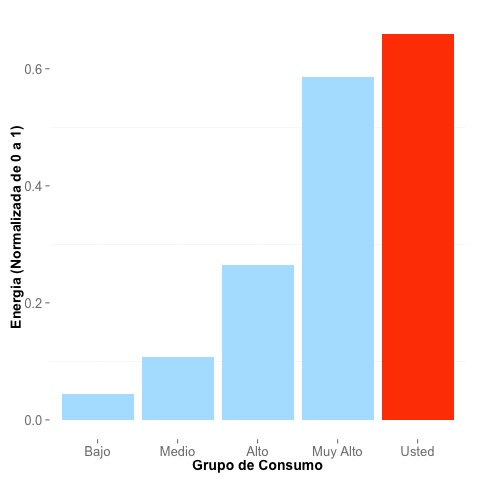
\includegraphics[scale=0.65]{figure/A1_neighbor_plot} 
\end{knitrout}

 \begin{textblock}{1}(9,-5)
\begin{minipage}{20em}
\begingroup
\input{A1_neighbor_plot.txt}
\endgroup
\end{minipage}
\end{textblock}


\begin{knitrout}
\definecolor{shadecolor}{rgb}{0.969, 0.969, 0.969}\color{fgcolor}
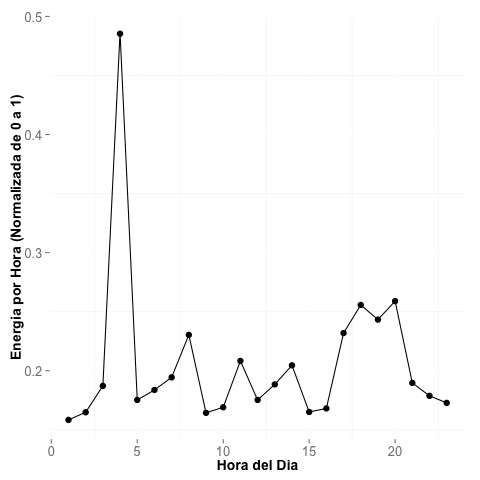
\includegraphics[scale=0.65]{figure/A1_plot_norm_median} 
\end{knitrout}


 \begin{textblock}{1}(9,-4)
\begin{minipage}{20em}
\begingroup
\input{A1_plot_norm_median.txt}
\endgroup
\end{minipage}
\end{textblock}


\begin{knitrout}
\definecolor{shadecolor}{rgb}{0.969, 0.969, 0.969}\color{fgcolor}
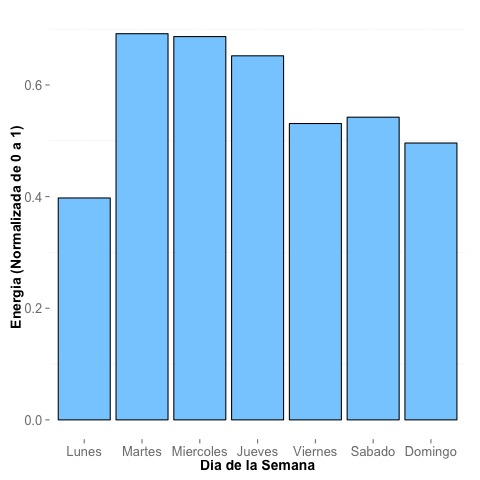
\includegraphics[scale=0.65]{figure/A1_day_of_week_plot} 
\end{knitrout}


 \begin{textblock}{1}(9,-3)
\begin{minipage}{20em}
\begingroup
\input{A1_day_of_week_plot.txt}
\endgroup
\end{minipage}
\end{textblock}


\begin{knitrout}
\definecolor{shadecolor}{rgb}{0.969, 0.969, 0.969}\color{fgcolor}
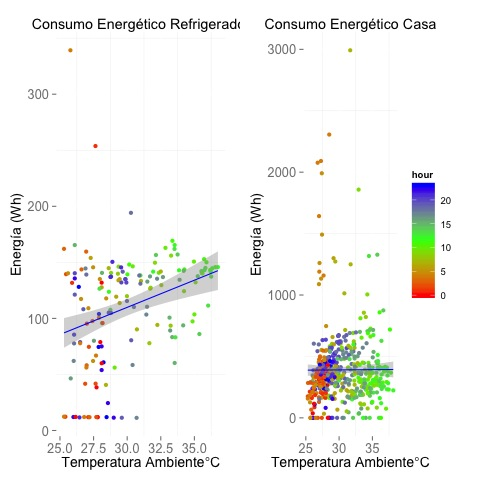
\includegraphics[scale=0.75]{figure/A1_correlaciones} 
\end{knitrout}

 \begin{textblock}{1}(9,-4)
\begin{minipage}{20em}
\begingroup
\input{A1_correlaciones.txt}
\endgroup
\end{minipage}
\end{textblock}


\vspace{70px}
\begin{knitrout}
Hola! Usted es parte de un estudio donde estamos tratando de entender como el consumo energetico de los hogares y las micro-empresas se puede mejor integrar a la red electrica de Nicaragua. Estamos utilizando los datos para desarrollar modelos de la red electrica, y tambien estamos tratando de entender como los datos energeticos pueden ser entregados a usted para que usted pueda mejor administrar su consumo y gasto energetico.  Estamos abiertos a sugerencias acerca de los datos y a maneras de que esto pueda ser de mejor uso para usted.
\end{knitrout}


\begin{knitrout}
\definecolor{shadecolor}{rgb}{0.969, 0.969, 0.969}\color{fgcolor}
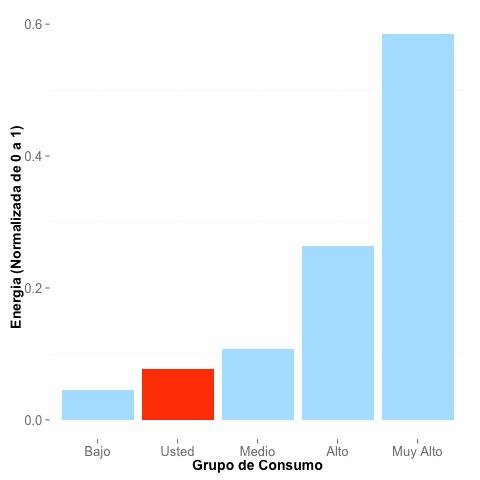
\includegraphics[scale=0.65]{figure/A2_neighbor_plot} 
\end{knitrout}

 \begin{textblock}{1}(9,-5)
\begin{minipage}{20em}
\begingroup
\input{A2_neighbor_plot.txt}
\endgroup
\end{minipage}
\end{textblock}


\begin{knitrout}
\definecolor{shadecolor}{rgb}{0.969, 0.969, 0.969}\color{fgcolor}
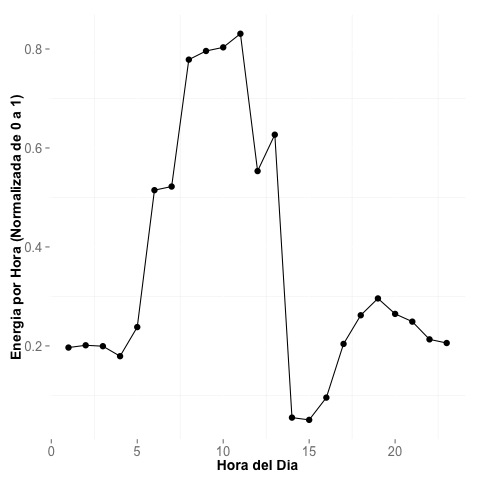
\includegraphics[scale=0.65]{figure/A2_plot_norm_median} 
\end{knitrout}


 \begin{textblock}{1}(9,-4)
\begin{minipage}{20em}
\begingroup
\input{A2_plot_norm_median.txt}
\endgroup
\end{minipage}
\end{textblock}


\begin{knitrout}
\definecolor{shadecolor}{rgb}{0.969, 0.969, 0.969}\color{fgcolor}
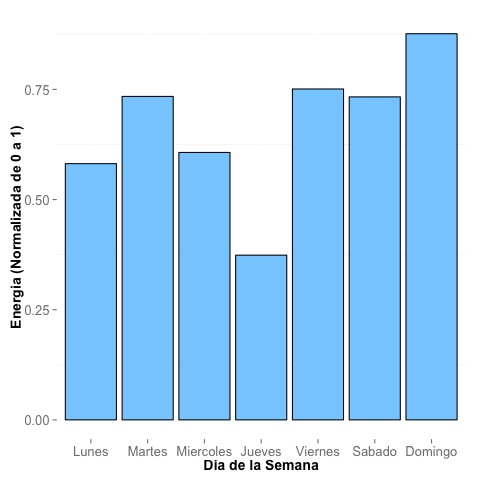
\includegraphics[scale=0.65]{figure/A2_day_of_week_plot} 
\end{knitrout}


 \begin{textblock}{1}(9,-3)
\begin{minipage}{20em}
\begingroup
\input{A2_day_of_week_plot.txt}
\endgroup
\end{minipage}
\end{textblock}


\begin{knitrout}
\definecolor{shadecolor}{rgb}{0.969, 0.969, 0.969}\color{fgcolor}
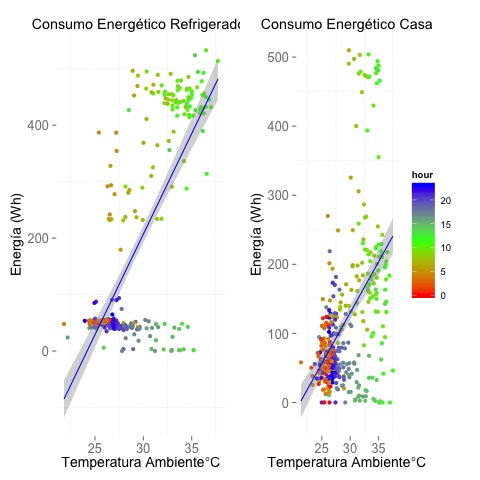
\includegraphics[scale=0.75]{figure/A2_correlaciones} 
\end{knitrout}

 \begin{textblock}{1}(9,-4)
\begin{minipage}{20em}
\begingroup
\input{A2_correlaciones.txt}
\endgroup
\end{minipage}
\end{textblock}

\vspace{70px}
\begin{knitrout}
Hola! Usted es parte de un estudio donde estamos tratando de entender como el consumo energetico de los hogares y las micro-empresas se puede mejor integrar a la red electrica de Nicaragua. Estamos utilizando los datos para desarrollar modelos de la red electrica, y tambien estamos tratando de entender como los datos energeticos pueden ser entregados a usted para que usted pueda mejor administrar su consumo y gasto energetico.  Estamos abiertos a sugerencias acerca de los datos y a maneras de que esto pueda ser de mejor uso para usted.
\end{knitrout}


\begin{knitrout}
\definecolor{shadecolor}{rgb}{0.969, 0.969, 0.969}\color{fgcolor}
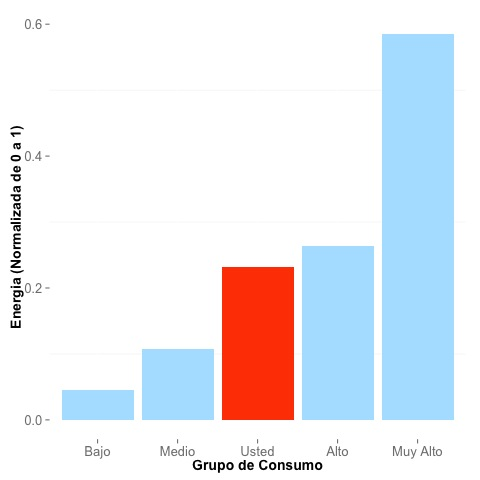
\includegraphics[scale=0.65]{figure/A3_neighbor_plot} 
\end{knitrout}

 \begin{textblock}{1}(9,-5)
\begin{minipage}{20em}
\begingroup
\input{A3_neighbor_plot.txt}
\endgroup
\end{minipage}
\end{textblock}


\begin{knitrout}
\definecolor{shadecolor}{rgb}{0.969, 0.969, 0.969}\color{fgcolor}
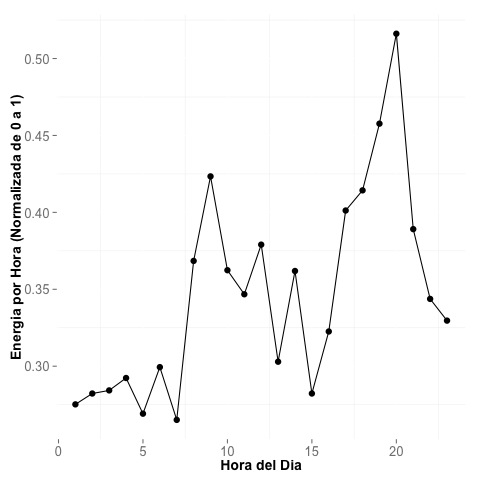
\includegraphics[scale=0.65]{figure/A3_plot_norm_median} 
\end{knitrout}


 \begin{textblock}{1}(9,-4)
\begin{minipage}{20em}
\begingroup
\input{A3_plot_norm_median.txt}
\endgroup
\end{minipage}
\end{textblock}


\begin{knitrout}
\definecolor{shadecolor}{rgb}{0.969, 0.969, 0.969}\color{fgcolor}
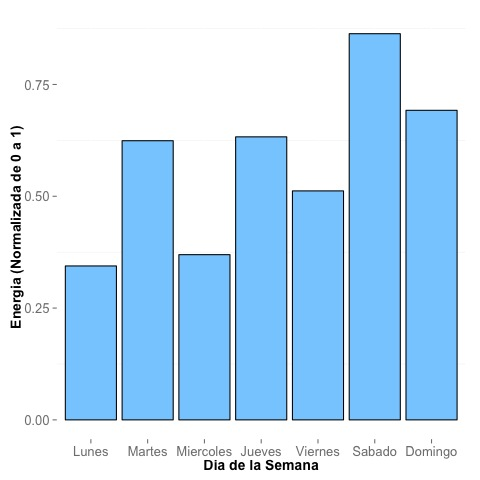
\includegraphics[scale=0.65]{figure/A3_day_of_week_plot} 
\end{knitrout}


 \begin{textblock}{1}(9,-3)
\begin{minipage}{20em}
\begingroup
\input{A3_day_of_week_plot.txt}
\endgroup
\end{minipage}
\end{textblock}


\begin{knitrout}
\definecolor{shadecolor}{rgb}{0.969, 0.969, 0.969}\color{fgcolor}
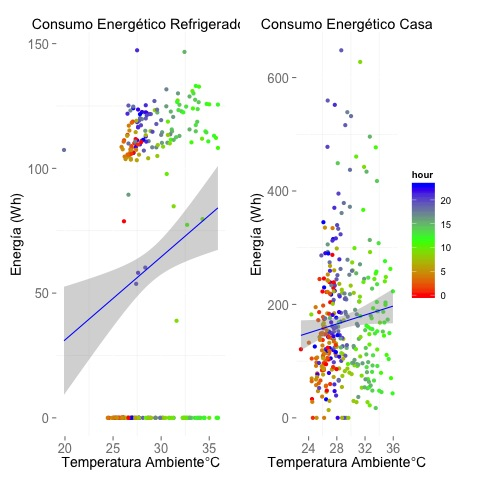
\includegraphics[scale=0.75]{figure/A3_correlaciones} 
\end{knitrout}

 \begin{textblock}{1}(9,-4)
\begin{minipage}{20em}
\begingroup
\input{A3_correlaciones.txt}
\endgroup
\end{minipage}
\end{textblock}

\vspace{70px}
\begin{knitrout}
Hola! Usted es parte de un estudio donde estamos tratando de entender como el consumo energetico de los hogares y las micro-empresas se puede mejor integrar a la red electrica de Nicaragua. Estamos utilizando los datos para desarrollar modelos de la red electrica, y tambien estamos tratando de entender como los datos energeticos pueden ser entregados a usted para que usted pueda mejor administrar su consumo y gasto energetico.  Estamos abiertos a sugerencias acerca de los datos y a maneras de que esto pueda ser de mejor uso para usted.
\end{knitrout}


\begin{knitrout}
\definecolor{shadecolor}{rgb}{0.969, 0.969, 0.969}\color{fgcolor}
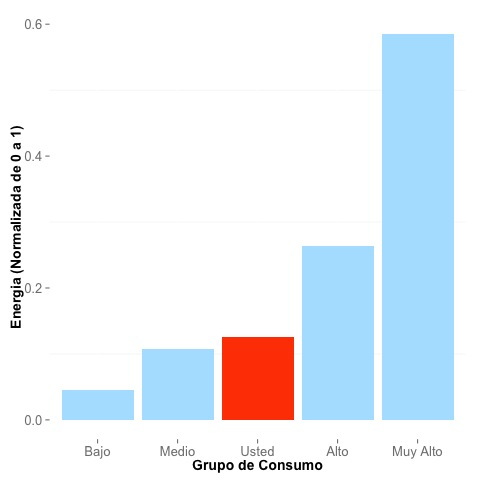
\includegraphics[scale=0.65]{figure/A4_neighbor_plot} 
\end{knitrout}

 \begin{textblock}{1}(9,-5)
\begin{minipage}{20em}
\begingroup
\input{A4_neighbor_plot.txt}
\endgroup
\end{minipage}
\end{textblock}


\begin{knitrout}
\definecolor{shadecolor}{rgb}{0.969, 0.969, 0.969}\color{fgcolor}
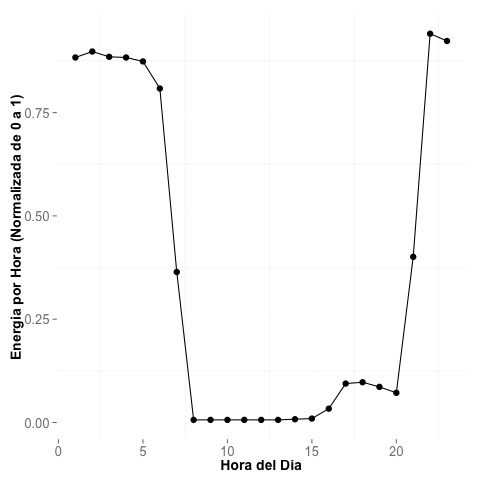
\includegraphics[scale=0.65]{figure/A4_plot_norm_median} 
\end{knitrout}


 \begin{textblock}{1}(9,-4)
\begin{minipage}{20em}
\begingroup
\input{A4_plot_norm_median.txt}
\endgroup
\end{minipage}
\end{textblock}


\begin{knitrout}
\definecolor{shadecolor}{rgb}{0.969, 0.969, 0.969}\color{fgcolor}
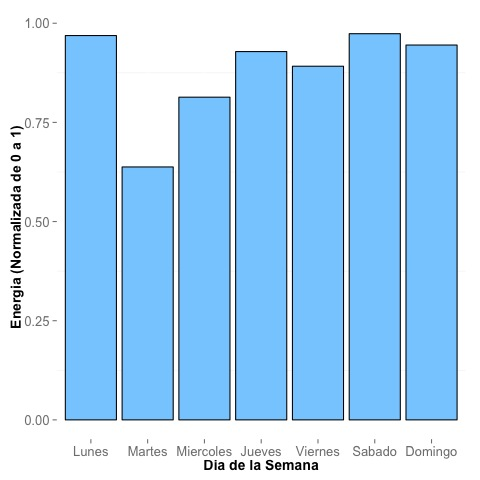
\includegraphics[scale=0.65]{figure/A4_day_of_week_plot} 
\end{knitrout}


 \begin{textblock}{1}(9,-3)
\begin{minipage}{20em}
\begingroup
\input{A4_day_of_week_plot.txt}
\endgroup
\end{minipage}
\end{textblock}


\begin{knitrout}
\definecolor{shadecolor}{rgb}{0.969, 0.969, 0.969}\color{fgcolor}
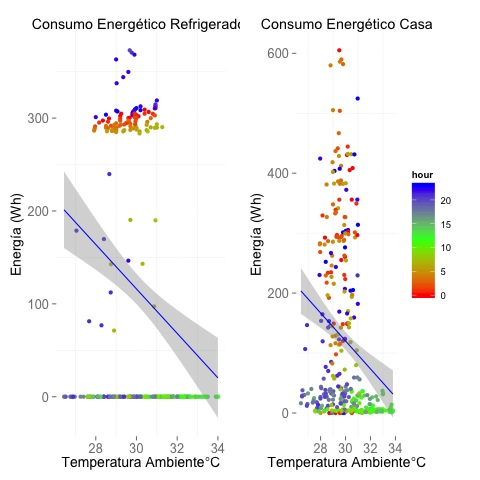
\includegraphics[scale=0.75]{figure/A4_correlaciones} 
\end{knitrout}

 \begin{textblock}{1}(9,-4)
\begin{minipage}{20em}
\begingroup
\input{A4_correlaciones.txt}
\endgroup
\end{minipage}
\end{textblock}

\vspace{70px}
\begin{knitrout}
Hola! Usted es parte de un estudio donde estamos tratando de entender como el consumo energetico de los hogares y las micro-empresas se puede mejor integrar a la red electrica de Nicaragua. Estamos utilizando los datos para desarrollar modelos de la red electrica, y tambien estamos tratando de entender como los datos energeticos pueden ser entregados a usted para que usted pueda mejor administrar su consumo y gasto energetico.  Estamos abiertos a sugerencias acerca de los datos y a maneras de que esto pueda ser de mejor uso para usted.
\end{knitrout}


\begin{knitrout}
\definecolor{shadecolor}{rgb}{0.969, 0.969, 0.969}\color{fgcolor}
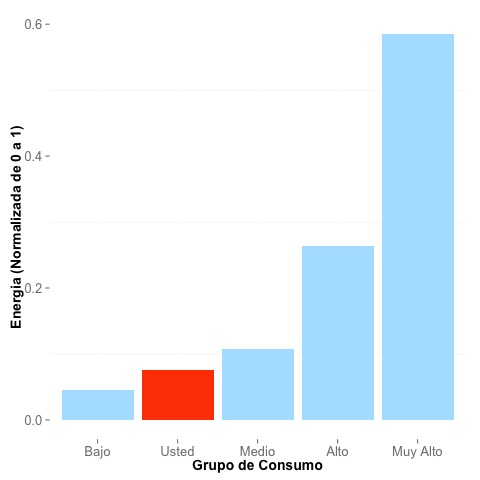
\includegraphics[scale=0.65]{figure/A5_neighbor_plot} 
\end{knitrout}

 \begin{textblock}{1}(9,-5)
\begin{minipage}{20em}
\begingroup
\input{A5_neighbor_plot.txt}
\endgroup
\end{minipage}
\end{textblock}


\begin{knitrout}
\definecolor{shadecolor}{rgb}{0.969, 0.969, 0.969}\color{fgcolor}
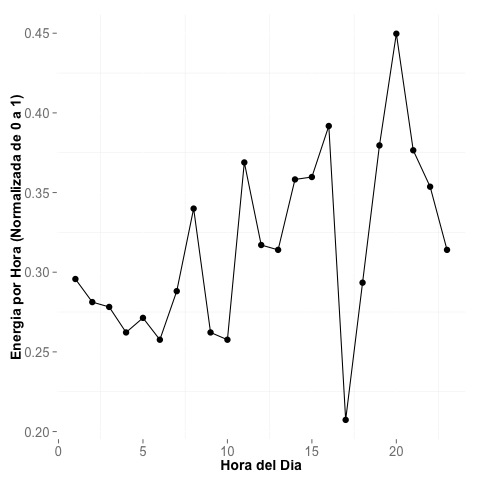
\includegraphics[scale=0.65]{figure/A5_plot_norm_median} 
\end{knitrout}


 \begin{textblock}{1}(9,-4)
\begin{minipage}{20em}
\begingroup
\input{A5_plot_norm_median.txt}
\endgroup
\end{minipage}
\end{textblock}


\begin{knitrout}
\definecolor{shadecolor}{rgb}{0.969, 0.969, 0.969}\color{fgcolor}
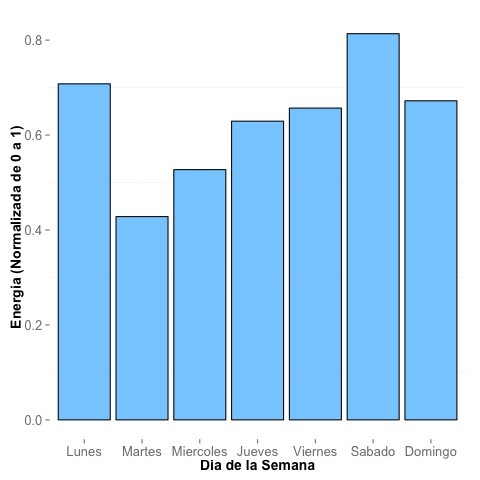
\includegraphics[scale=0.65]{figure/A5_day_of_week_plot} 
\end{knitrout}


 \begin{textblock}{1}(9,-3)
\begin{minipage}{20em}
\begingroup
\input{A5_day_of_week_plot.txt}
\endgroup
\end{minipage}
\end{textblock}


\begin{knitrout}
\definecolor{shadecolor}{rgb}{0.969, 0.969, 0.969}\color{fgcolor}
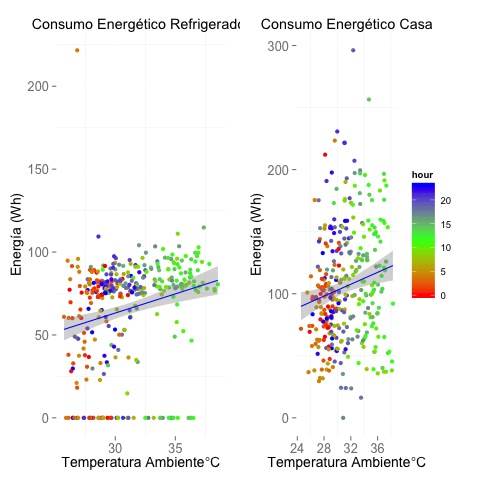
\includegraphics[scale=0.75]{figure/A5_correlaciones} 
\end{knitrout}

 \begin{textblock}{1}(9,-4)
\begin{minipage}{20em}
\begingroup
\input{A5_correlaciones.txt}
\endgroup
\end{minipage}
\end{textblock}

\vspace{70px}
\begin{knitrout}
Hola! Usted es parte de un estudio donde estamos tratando de entender como el consumo energetico de los hogares y las micro-empresas se puede mejor integrar a la red electrica de Nicaragua. Estamos utilizando los datos para desarrollar modelos de la red electrica, y tambien estamos tratando de entender como los datos energeticos pueden ser entregados a usted para que usted pueda mejor administrar su consumo y gasto energetico.  Estamos abiertos a sugerencias acerca de los datos y a maneras de que esto pueda ser de mejor uso para usted.
\end{knitrout}


\begin{knitrout}
\definecolor{shadecolor}{rgb}{0.969, 0.969, 0.969}\color{fgcolor}
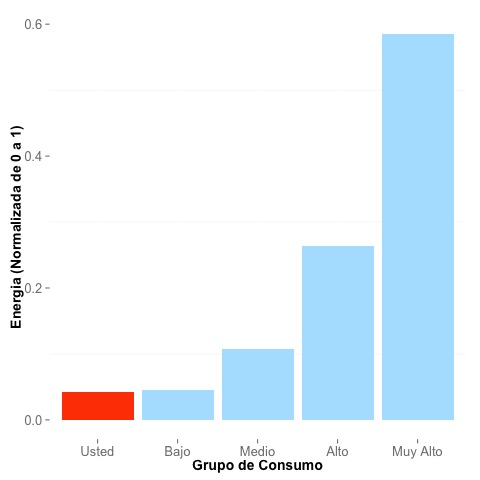
\includegraphics[scale=0.65]{figure/A6_neighbor_plot} 
\end{knitrout}

 \begin{textblock}{1}(9,-5)
\begin{minipage}{20em}
\begingroup
\input{A6_neighbor_plot.txt}
\endgroup
\end{minipage}
\end{textblock}


\begin{knitrout}
\definecolor{shadecolor}{rgb}{0.969, 0.969, 0.969}\color{fgcolor}
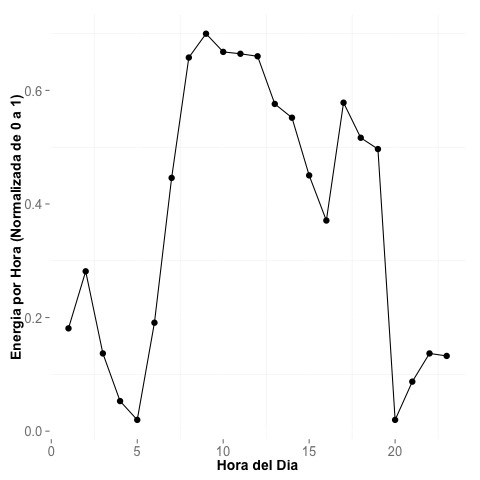
\includegraphics[scale=0.65]{figure/A6_plot_norm_median} 
\end{knitrout}


 \begin{textblock}{1}(9,-4)
\begin{minipage}{20em}
\begingroup
\input{A6_plot_norm_median.txt}
\endgroup
\end{minipage}
\end{textblock}


\begin{knitrout}
\definecolor{shadecolor}{rgb}{0.969, 0.969, 0.969}\color{fgcolor}
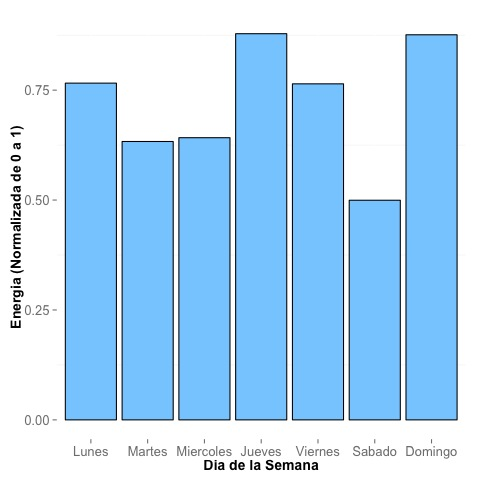
\includegraphics[scale=0.65]{figure/A6_day_of_week_plot} 
\end{knitrout}


 \begin{textblock}{1}(9,-3)
\begin{minipage}{20em}
\begingroup
\input{A6_day_of_week_plot.txt}
\endgroup
\end{minipage}
\end{textblock}


\begin{knitrout}
\definecolor{shadecolor}{rgb}{0.969, 0.969, 0.969}\color{fgcolor}
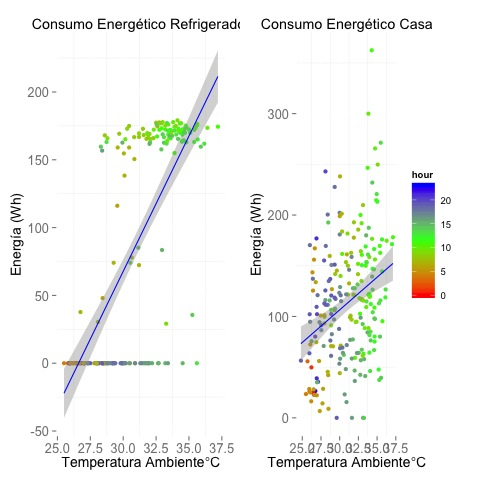
\includegraphics[scale=0.75]{figure/A6_correlaciones} 
\end{knitrout}

 \begin{textblock}{1}(9,-4)
\begin{minipage}{20em}
\begingroup
\input{A6_correlaciones.txt}
\endgroup
\end{minipage}
\end{textblock}


\vspace{70px}
\begin{knitrout}
Hola! Usted es parte de un estudio donde estamos tratando de entender como el consumo energetico de los hogares y las micro-empresas se puede mejor integrar a la red electrica de Nicaragua. Estamos utilizando los datos para desarrollar modelos de la red electrica, y tambien estamos tratando de entender como los datos energeticos pueden ser entregados a usted para que usted pueda mejor administrar su consumo y gasto energetico.  Estamos abiertos a sugerencias acerca de los datos y a maneras de que esto pueda ser de mejor uso para usted.
\end{knitrout}


\begin{knitrout}
\definecolor{shadecolor}{rgb}{0.969, 0.969, 0.969}\color{fgcolor}
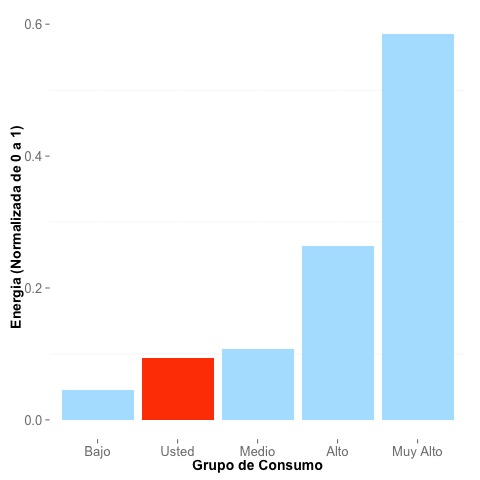
\includegraphics[scale=0.65]{figure/A7_neighbor_plot} 
\end{knitrout}

 \begin{textblock}{1}(9,-5)
\begin{minipage}{20em}
\begingroup
\input{A7_neighbor_plot.txt}
\endgroup
\end{minipage}
\end{textblock}


\begin{knitrout}
\definecolor{shadecolor}{rgb}{0.969, 0.969, 0.969}\color{fgcolor}
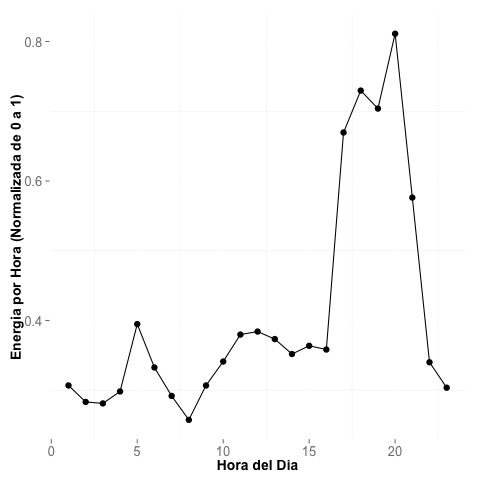
\includegraphics[scale=0.65]{figure/A7_plot_norm_median} 
\end{knitrout}


 \begin{textblock}{1}(9,-4)
\begin{minipage}{20em}
\begingroup
\input{A7_plot_norm_median.txt}
\endgroup
\end{minipage}
\end{textblock}


\begin{knitrout}
\definecolor{shadecolor}{rgb}{0.969, 0.969, 0.969}\color{fgcolor}
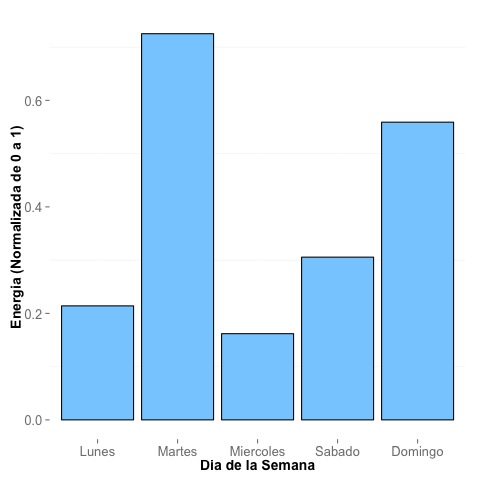
\includegraphics[scale=0.65]{figure/A7_day_of_week_plot} 
\end{knitrout}


 \begin{textblock}{1}(9,-3)
\begin{minipage}{20em}
\begingroup
\input{A7_day_of_week_plot.txt}
\endgroup
\end{minipage}
\end{textblock}


\begin{knitrout}
\definecolor{shadecolor}{rgb}{0.969, 0.969, 0.969}\color{fgcolor}
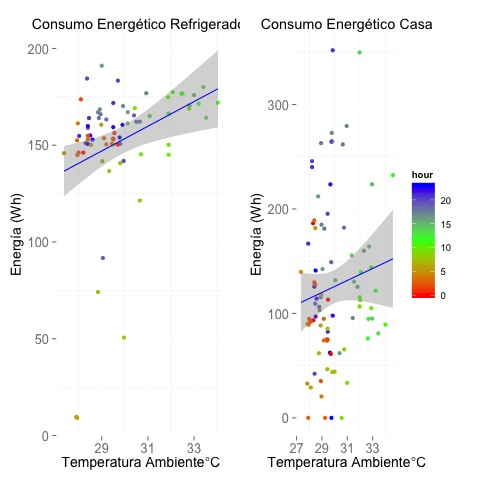
\includegraphics[scale=0.75]{figure/A7_correlaciones} 
\end{knitrout}

 \begin{textblock}{1}(9,-4)
\begin{minipage}{20em}
\begingroup
\input{A7_correlaciones.txt}
\endgroup
\end{minipage}
\end{textblock}

\vspace{70px}
\begin{knitrout}
Hola! Usted es parte de un estudio donde estamos tratando de entender como el consumo energetico de los hogares y las micro-empresas se puede mejor integrar a la red electrica de Nicaragua. Estamos utilizando los datos para desarrollar modelos de la red electrica, y tambien estamos tratando de entender como los datos energeticos pueden ser entregados a usted para que usted pueda mejor administrar su consumo y gasto energetico.  Estamos abiertos a sugerencias acerca de los datos y a maneras de que esto pueda ser de mejor uso para usted.
\end{knitrout}


\begin{knitrout}
\definecolor{shadecolor}{rgb}{0.969, 0.969, 0.969}\color{fgcolor}
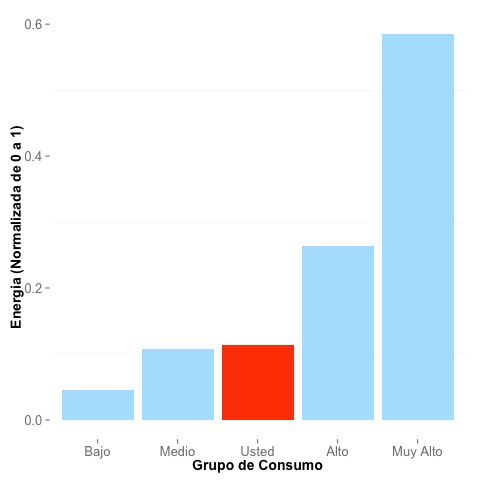
\includegraphics[scale=0.65]{figure/A8_neighbor_plot} 
\end{knitrout}

 \begin{textblock}{1}(9,-5)
\begin{minipage}{20em}
\begingroup
\input{A8_neighbor_plot.txt}
\endgroup
\end{minipage}
\end{textblock}


\begin{knitrout}
\definecolor{shadecolor}{rgb}{0.969, 0.969, 0.969}\color{fgcolor}
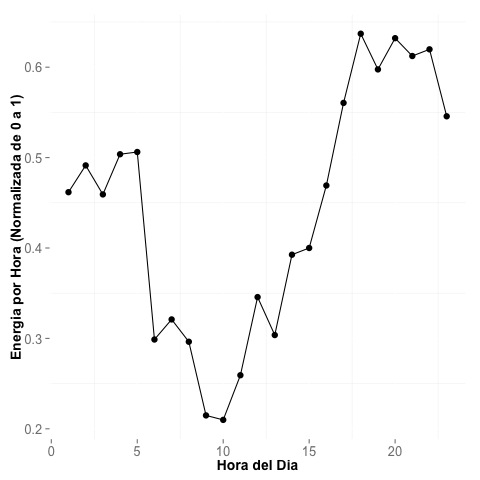
\includegraphics[scale=0.65]{figure/A8_plot_norm_median} 
\end{knitrout}


 \begin{textblock}{1}(9,-4)
\begin{minipage}{20em}
\begingroup
\input{A8_plot_norm_median.txt}
\endgroup
\end{minipage}
\end{textblock}


\begin{knitrout}
\definecolor{shadecolor}{rgb}{0.969, 0.969, 0.969}\color{fgcolor}
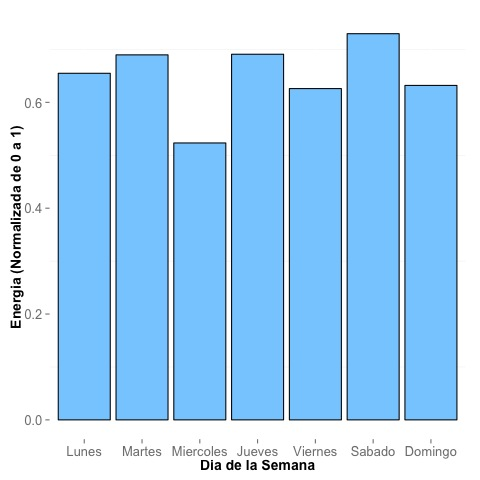
\includegraphics[scale=0.65]{figure/A8_day_of_week_plot} 
\end{knitrout}


 \begin{textblock}{1}(9,-3)
\begin{minipage}{20em}
\begingroup
\input{A8_day_of_week_plot.txt}
\endgroup
\end{minipage}
\end{textblock}


\begin{knitrout}
\definecolor{shadecolor}{rgb}{0.969, 0.969, 0.969}\color{fgcolor}
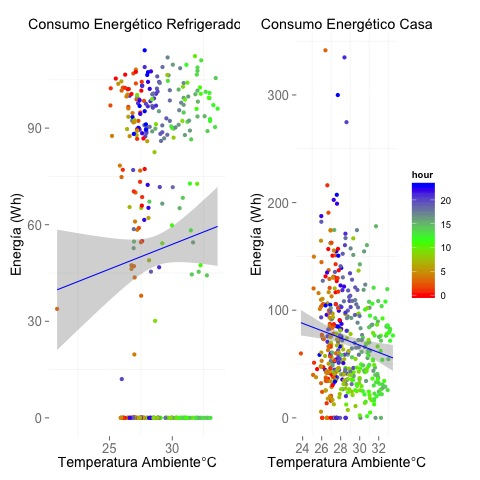
\includegraphics[scale=0.75]{figure/A8_correlaciones} 
\end{knitrout}

 \begin{textblock}{1}(9,-4)
\begin{minipage}{20em}
\begingroup
\input{A8_correlaciones.txt}
\endgroup
\end{minipage}
\end{textblock}

\vspace{70px}
\begin{knitrout}
Hola! Usted es parte de un estudio donde estamos tratando de entender como el consumo energetico de los hogares y las micro-empresas se puede mejor integrar a la red electrica de Nicaragua. Estamos utilizando los datos para desarrollar modelos de la red electrica, y tambien estamos tratando de entender como los datos energeticos pueden ser entregados a usted para que usted pueda mejor administrar su consumo y gasto energetico.  Estamos abiertos a sugerencias acerca de los datos y a maneras de que esto pueda ser de mejor uso para usted.
\end{knitrout}


\begin{knitrout}
\definecolor{shadecolor}{rgb}{0.969, 0.969, 0.969}\color{fgcolor}
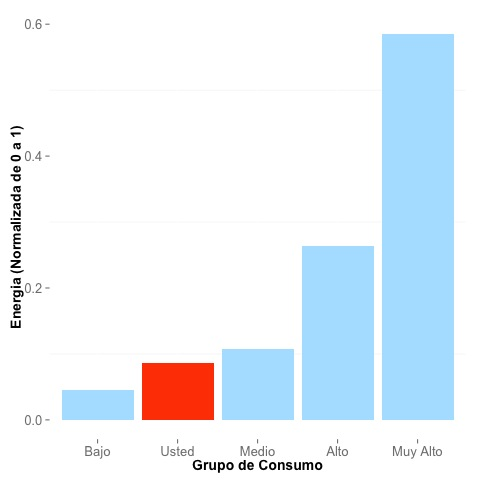
\includegraphics[scale=0.65]{figure/A9_neighbor_plot} 
\end{knitrout}

 \begin{textblock}{1}(9,-5)
\begin{minipage}{20em}
\begingroup
\input{A9_neighbor_plot.txt}
\endgroup
\end{minipage}
\end{textblock}


\begin{knitrout}
\definecolor{shadecolor}{rgb}{0.969, 0.969, 0.969}\color{fgcolor}
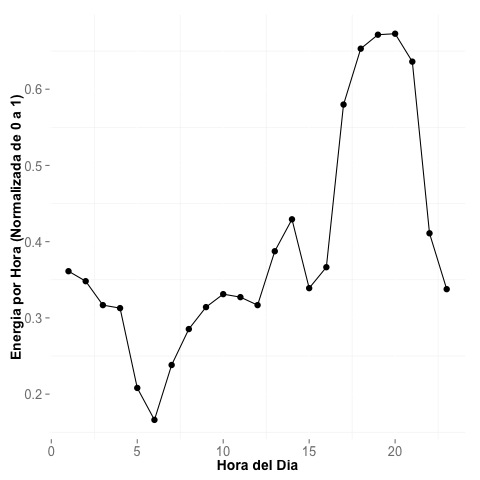
\includegraphics[scale=0.65]{figure/A9_plot_norm_median} 
\end{knitrout}


 \begin{textblock}{1}(9,-4)
\begin{minipage}{20em}
\begingroup
\input{A9_plot_norm_median.txt}
\endgroup
\end{minipage}
\end{textblock}


\begin{knitrout}
\definecolor{shadecolor}{rgb}{0.969, 0.969, 0.969}\color{fgcolor}
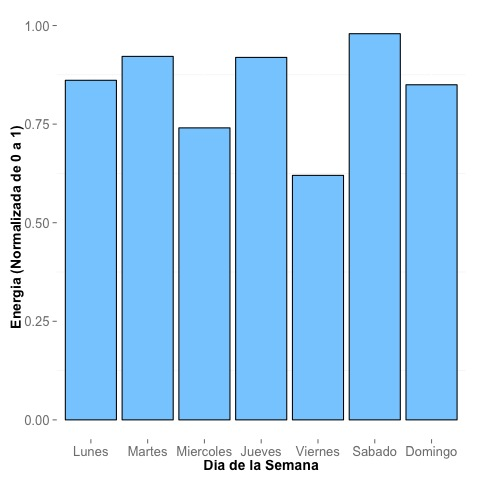
\includegraphics[scale=0.65]{figure/A9_day_of_week_plot} 
\end{knitrout}


 \begin{textblock}{1}(9,-3)
\begin{minipage}{20em}
\begingroup
\input{A9_day_of_week_plot.txt}
\endgroup
\end{minipage}
\end{textblock}


\begin{knitrout}
\definecolor{shadecolor}{rgb}{0.969, 0.969, 0.969}\color{fgcolor}
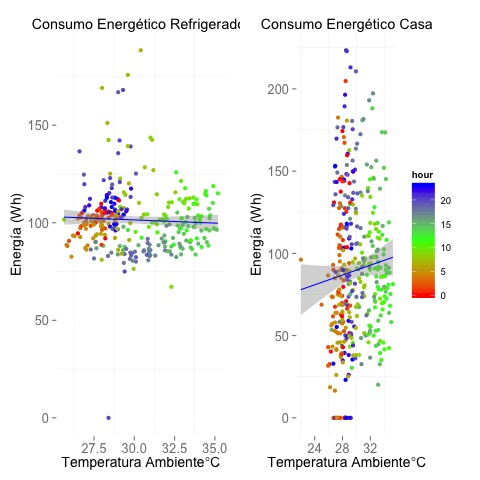
\includegraphics[scale=0.75]{figure/A9_correlaciones} 
\end{knitrout}

 \begin{textblock}{1}(9,-4)
\begin{minipage}{20em}
\begingroup
\input{A9_correlaciones.txt}
\endgroup
\end{minipage}
\end{textblock}

\vspace{70px}
\begin{knitrout}
Hola! Usted es parte de un estudio donde estamos tratando de entender como el consumo energetico de los hogares y las micro-empresas se puede mejor integrar a la red electrica de Nicaragua. Estamos utilizando los datos para desarrollar modelos de la red electrica, y tambien estamos tratando de entender como los datos energeticos pueden ser entregados a usted para que usted pueda mejor administrar su consumo y gasto energetico.  Estamos abiertos a sugerencias acerca de los datos y a maneras de que esto pueda ser de mejor uso para usted.
\end{knitrout}


\begin{knitrout}
\definecolor{shadecolor}{rgb}{0.969, 0.969, 0.969}\color{fgcolor}
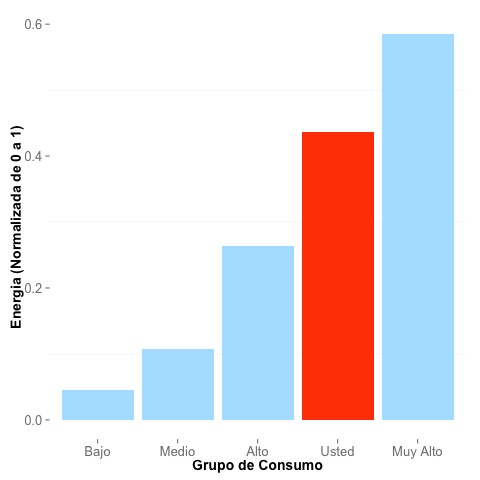
\includegraphics[scale=0.65]{figure/A10_neighbor_plot} 
\end{knitrout}

 \begin{textblock}{1}(9,-5)
\begin{minipage}{20em}
\begingroup
\input{A10_neighbor_plot.txt}
\endgroup
\end{minipage}
\end{textblock}


\begin{knitrout}
\definecolor{shadecolor}{rgb}{0.969, 0.969, 0.969}\color{fgcolor}
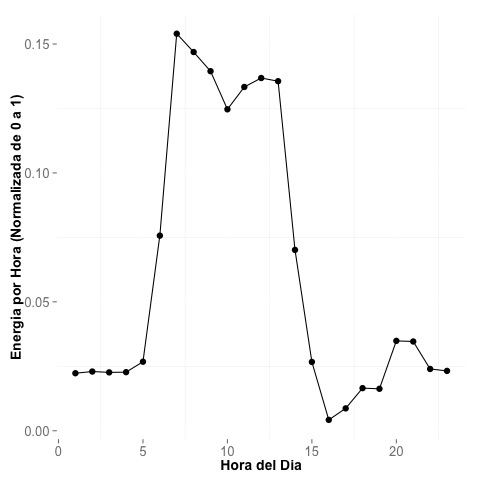
\includegraphics[scale=0.65]{figure/A10_plot_norm_median} 
\end{knitrout}


 \begin{textblock}{1}(9,-4)
\begin{minipage}{20em}
\begingroup
\input{A10_plot_norm_median.txt}
\endgroup
\end{minipage}
\end{textblock}


\begin{knitrout}
\definecolor{shadecolor}{rgb}{0.969, 0.969, 0.969}\color{fgcolor}
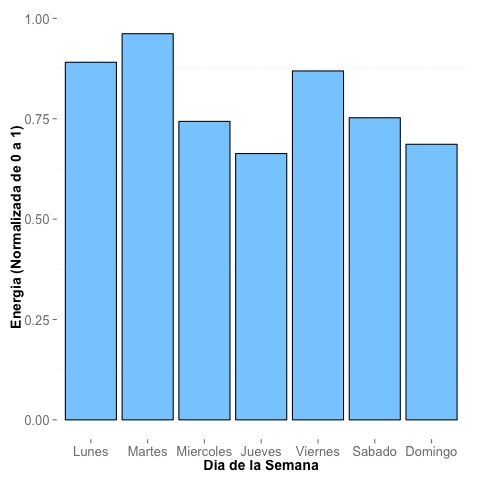
\includegraphics[scale=0.65]{figure/A10_day_of_week_plot} 
\end{knitrout}


 \begin{textblock}{1}(9,-3)
\begin{minipage}{20em}
\begingroup
\input{A10_day_of_week_plot.txt}
\endgroup
\end{minipage}
\end{textblock}


\begin{knitrout}
\definecolor{shadecolor}{rgb}{0.969, 0.969, 0.969}\color{fgcolor}
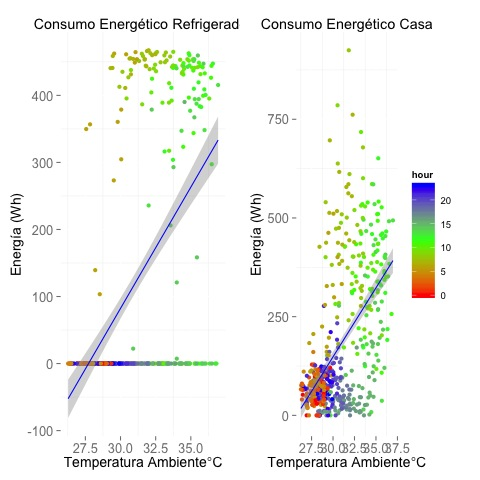
\includegraphics[scale=0.75]{figure/A10_correlaciones} 
\end{knitrout}

 \begin{textblock}{1}(9,-4)
\begin{minipage}{20em}
\begingroup
\input{A10_correlaciones.txt}
\endgroup
\end{minipage}
\end{textblock}

\vspace{70px}
\begin{knitrout}
Hola! Usted es parte de un estudio donde estamos tratando de entender como el consumo energetico de los hogares y las micro-empresas se puede mejor integrar a la red electrica de Nicaragua. Estamos utilizando los datos para desarrollar modelos de la red electrica, y tambien estamos tratando de entender como los datos energeticos pueden ser entregados a usted para que usted pueda mejor administrar su consumo y gasto energetico.  Estamos abiertos a sugerencias acerca de los datos y a maneras de que esto pueda ser de mejor uso para usted.
\end{knitrout}


\begin{knitrout}
\definecolor{shadecolor}{rgb}{0.969, 0.969, 0.969}\color{fgcolor}
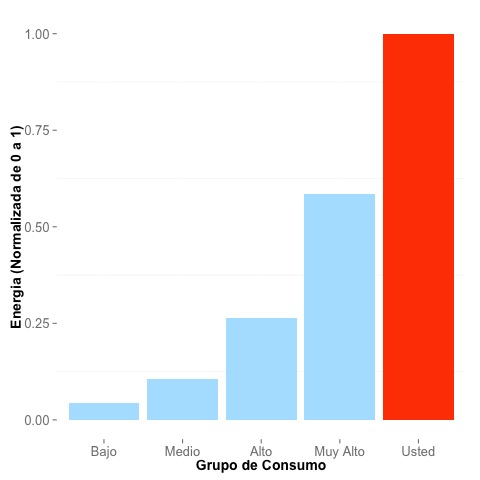
\includegraphics[scale=0.65]{figure/A11_neighbor_plot} 
\end{knitrout}

 \begin{textblock}{1}(9,-5)
\begin{minipage}{20em}
\begingroup
\input{A11_neighbor_plot.txt}
\endgroup
\end{minipage}
\end{textblock}


\begin{knitrout}
\definecolor{shadecolor}{rgb}{0.969, 0.969, 0.969}\color{fgcolor}
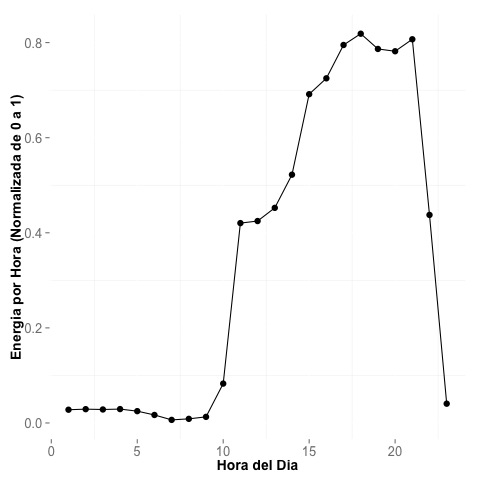
\includegraphics[scale=0.65]{figure/A11_plot_norm_median} 
\end{knitrout}


 \begin{textblock}{1}(9,-4)
\begin{minipage}{20em}
\begingroup
\input{A11_plot_norm_median.txt}
\endgroup
\end{minipage}
\end{textblock}


\begin{knitrout}
\definecolor{shadecolor}{rgb}{0.969, 0.969, 0.969}\color{fgcolor}
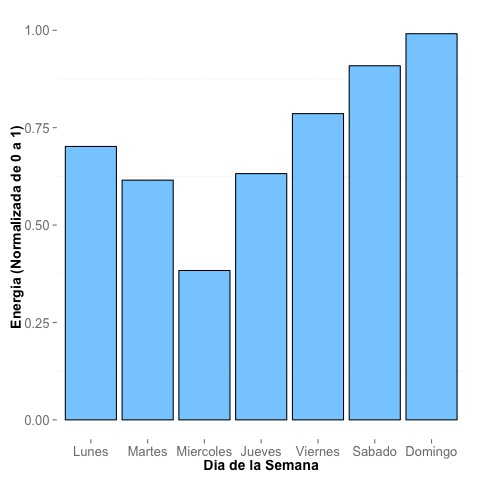
\includegraphics[scale=0.65]{figure/A11_day_of_week_plot} 
\end{knitrout}


 \begin{textblock}{1}(9,-3)
\begin{minipage}{20em}
\begingroup
\input{A11_day_of_week_plot.txt}
\endgroup
\end{minipage}
\end{textblock}


\begin{knitrout}
\definecolor{shadecolor}{rgb}{0.969, 0.969, 0.969}\color{fgcolor}
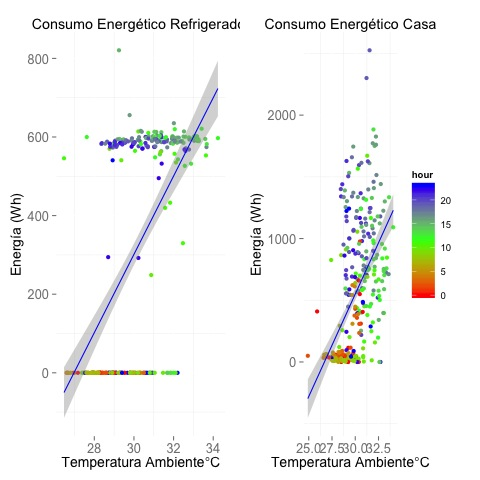
\includegraphics[scale=0.75]{figure/A11_correlaciones} 
\end{knitrout}

 \begin{textblock}{1}(9,-4)
\begin{minipage}{20em}
\begingroup
\input{A11_correlaciones.txt}
\endgroup
\end{minipage}
\end{textblock}

\vspace{70px}
\begin{knitrout}
Hola! Usted es parte de un estudio donde estamos tratando de entender como el consumo energetico de los hogares y las micro-empresas se puede mejor integrar a la red electrica de Nicaragua. Estamos utilizando los datos para desarrollar modelos de la red electrica, y tambien estamos tratando de entender como los datos energeticos pueden ser entregados a usted para que usted pueda mejor administrar su consumo y gasto energetico.  Estamos abiertos a sugerencias acerca de los datos y a maneras de que esto pueda ser de mejor uso para usted.
\end{knitrout}


\begin{knitrout}
\definecolor{shadecolor}{rgb}{0.969, 0.969, 0.969}\color{fgcolor}
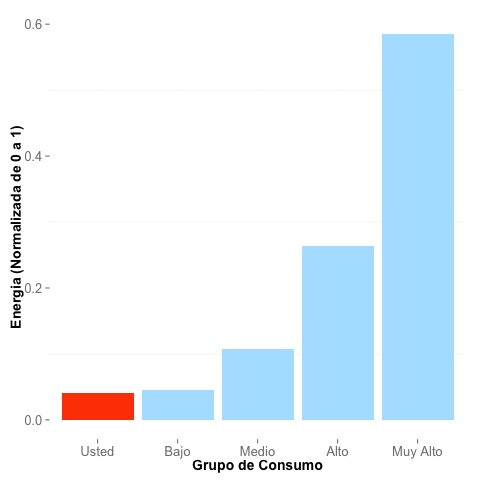
\includegraphics[scale=0.65]{figure/A12_neighbor_plot} 
\end{knitrout}

 \begin{textblock}{1}(9,-5)
\begin{minipage}{20em}
\begingroup
\input{A12_neighbor_plot.txt}
\endgroup
\end{minipage}
\end{textblock}


\begin{knitrout}
\definecolor{shadecolor}{rgb}{0.969, 0.969, 0.969}\color{fgcolor}
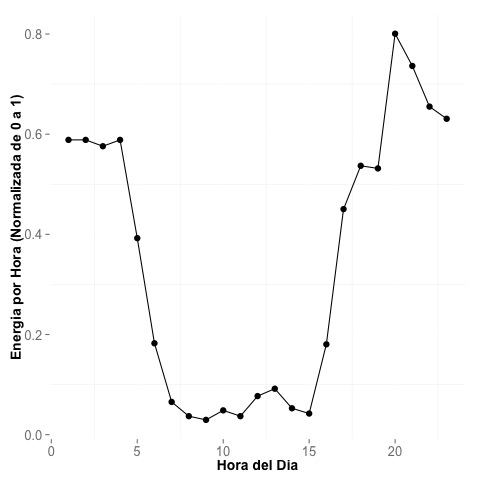
\includegraphics[scale=0.65]{figure/A12_plot_norm_median} 
\end{knitrout}


 \begin{textblock}{1}(9,-4)
\begin{minipage}{20em}
\begingroup
\input{A12_plot_norm_median.txt}
\endgroup
\end{minipage}
\end{textblock}


\begin{knitrout}
\definecolor{shadecolor}{rgb}{0.969, 0.969, 0.969}\color{fgcolor}
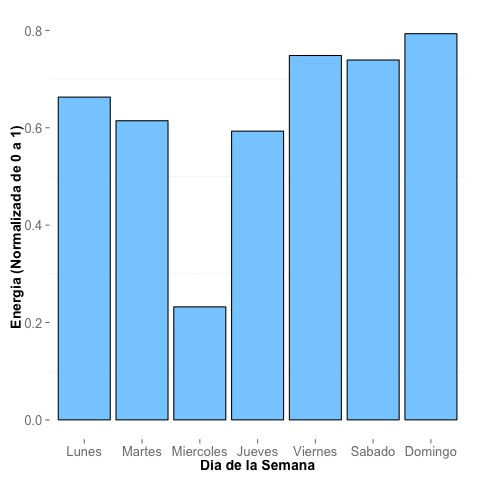
\includegraphics[scale=0.65]{figure/A12_day_of_week_plot} 
\end{knitrout}


 \begin{textblock}{1}(9,-3)
\begin{minipage}{20em}
\begingroup
\input{A12_day_of_week_plot.txt}
\endgroup
\end{minipage}
\end{textblock}


\begin{knitrout}
\definecolor{shadecolor}{rgb}{0.969, 0.969, 0.969}\color{fgcolor}
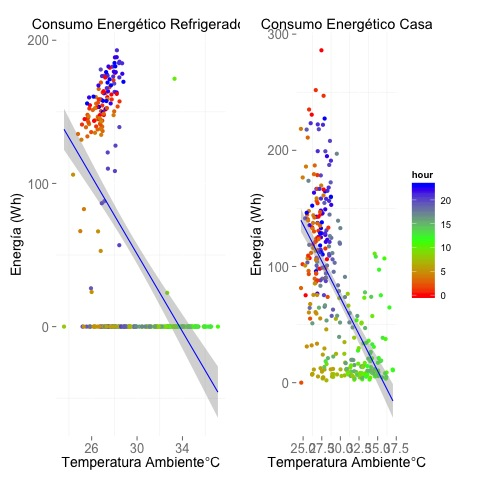
\includegraphics[scale=0.75]{figure/A12_correlaciones} 
\end{knitrout}

 \begin{textblock}{1}(9,-4)
\begin{minipage}{20em}
\begingroup
\input{A12_correlaciones.txt}
\endgroup
\end{minipage}
\end{textblock}

\vspace{70px}
\begin{knitrout}
Hola! Usted es parte de un estudio donde estamos tratando de entender como el consumo energetico de los hogares y las micro-empresas se puede mejor integrar a la red electrica de Nicaragua. Estamos utilizando los datos para desarrollar modelos de la red electrica, y tambien estamos tratando de entender como los datos energeticos pueden ser entregados a usted para que usted pueda mejor administrar su consumo y gasto energetico.  Estamos abiertos a sugerencias acerca de los datos y a maneras de que esto pueda ser de mejor uso para usted.
\end{knitrout}


\begin{knitrout}
\definecolor{shadecolor}{rgb}{0.969, 0.969, 0.969}\color{fgcolor}
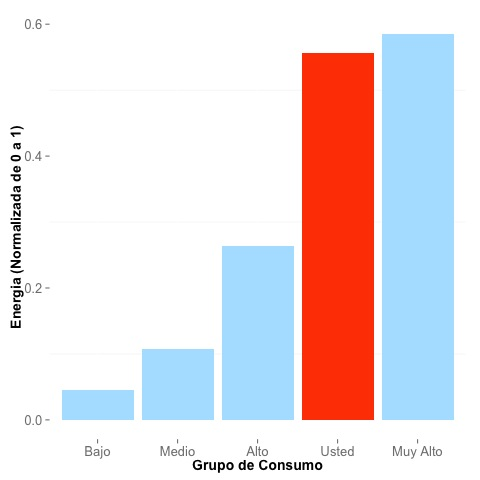
\includegraphics[scale=0.65]{figure/A13_neighbor_plot} 
\end{knitrout}

 \begin{textblock}{1}(9,-5)
\begin{minipage}{20em}
\begingroup
\input{A13_neighbor_plot.txt}
\endgroup
\end{minipage}
\end{textblock}


\begin{knitrout}
\definecolor{shadecolor}{rgb}{0.969, 0.969, 0.969}\color{fgcolor}
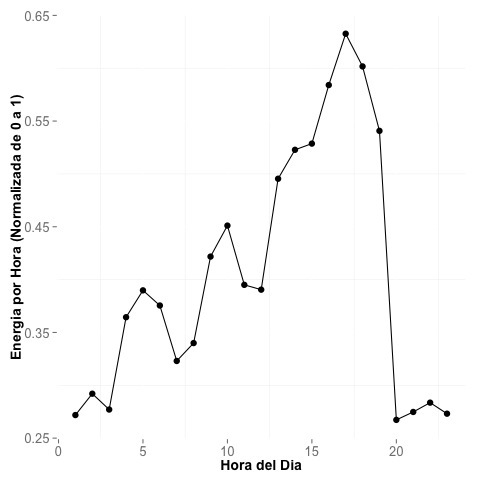
\includegraphics[scale=0.65]{figure/A13_plot_norm_median} 
\end{knitrout}


 \begin{textblock}{1}(9,-4)
\begin{minipage}{20em}
\begingroup
\input{A13_plot_norm_median.txt}
\endgroup
\end{minipage}
\end{textblock}


\begin{knitrout}
\definecolor{shadecolor}{rgb}{0.969, 0.969, 0.969}\color{fgcolor}
\includegraphics[scale=0.65]{figure/A13_day_of_week_plot} 
\end{knitrout}


 \begin{textblock}{1}(9,-3)
\begin{minipage}{20em}
\begingroup
\input{A13_day_of_week_plot.txt}
\endgroup
\end{minipage}
\end{textblock}


\begin{knitrout}
\definecolor{shadecolor}{rgb}{0.969, 0.969, 0.969}\color{fgcolor}
\includegraphics[scale=0.75]{figure/A13_correlaciones} 
\end{knitrout}

 \begin{textblock}{1}(9,-4)
\begin{minipage}{20em}
\begingroup
\input{A13_correlaciones.txt}
\endgroup
\end{minipage}
\end{textblock}

\vspace{70px}
\begin{knitrout}
Hola! Usted es parte de un estudio donde estamos tratando de entender como el consumo energetico de los hogares y las micro-empresas se puede mejor integrar a la red electrica de Nicaragua. Estamos utilizando los datos para desarrollar modelos de la red electrica, y tambien estamos tratando de entender como los datos energeticos pueden ser entregados a usted para que usted pueda mejor administrar su consumo y gasto energetico.  Estamos abiertos a sugerencias acerca de los datos y a maneras de que esto pueda ser de mejor uso para usted.
\end{knitrout}


\begin{knitrout}
\definecolor{shadecolor}{rgb}{0.969, 0.969, 0.969}\color{fgcolor}
\includegraphics[scale=0.65]{figure/A14_neighbor_plot} 
\end{knitrout}

 \begin{textblock}{1}(9,-5)
\begin{minipage}{20em}
\begingroup
\input{A14_neighbor_plot.txt}
\endgroup
\end{minipage}
\end{textblock}


\begin{knitrout}
\definecolor{shadecolor}{rgb}{0.969, 0.969, 0.969}\color{fgcolor}
\includegraphics[scale=0.65]{figure/A14_plot_norm_median} 
\end{knitrout}


 \begin{textblock}{1}(9,-4)
\begin{minipage}{20em}
\begingroup
\input{A14_plot_norm_median.txt}
\endgroup
\end{minipage}
\end{textblock}


\begin{knitrout}
\definecolor{shadecolor}{rgb}{0.969, 0.969, 0.969}\color{fgcolor}
\includegraphics[scale=0.65]{figure/A14_day_of_week_plot} 
\end{knitrout}


 \begin{textblock}{1}(9,-3)
\begin{minipage}{20em}
\begingroup
\input{A14_day_of_week_plot.txt}
\endgroup
\end{minipage}
\end{textblock}


\begin{knitrout}
\definecolor{shadecolor}{rgb}{0.969, 0.969, 0.969}\color{fgcolor}
\includegraphics[scale=0.75]{figure/A14_correlaciones} 
\end{knitrout}

 \begin{textblock}{1}(9,-4)
\begin{minipage}{20em}
\begingroup
\input{A14_correlaciones.txt}
\endgroup
\end{minipage}
\end{textblock}

\vspace{70px}
\begin{knitrout}
Hola! Usted es parte de un estudio donde estamos tratando de entender como el consumo energetico de los hogares y las micro-empresas se puede mejor integrar a la red electrica de Nicaragua. Estamos utilizando los datos para desarrollar modelos de la red electrica, y tambien estamos tratando de entender como los datos energeticos pueden ser entregados a usted para que usted pueda mejor administrar su consumo y gasto energetico.  Estamos abiertos a sugerencias acerca de los datos y a maneras de que esto pueda ser de mejor uso para usted.
\end{knitrout}


\begin{knitrout}
\definecolor{shadecolor}{rgb}{0.969, 0.969, 0.969}\color{fgcolor}
\includegraphics[scale=0.65]{figure/A15_neighbor_plot} 
\end{knitrout}

 \begin{textblock}{1}(9,-5)
\begin{minipage}{20em}
\begingroup
\input{A15_neighbor_plot.txt}
\endgroup
\end{minipage}
\end{textblock}


\begin{knitrout}
\definecolor{shadecolor}{rgb}{0.969, 0.969, 0.969}\color{fgcolor}
\includegraphics[scale=0.65]{figure/A15_plot_norm_median} 
\end{knitrout}


 \begin{textblock}{1}(9,-4)
\begin{minipage}{20em}
\begingroup
\input{A15_plot_norm_median.txt}
\endgroup
\end{minipage}
\end{textblock}


\begin{knitrout}
\definecolor{shadecolor}{rgb}{0.969, 0.969, 0.969}\color{fgcolor}
\includegraphics[scale=0.65]{figure/A15_day_of_week_plot} 
\end{knitrout}


 \begin{textblock}{1}(9,-3)
\begin{minipage}{20em}
\begingroup
\input{A15_day_of_week_plot.txt}
\endgroup
\end{minipage}
\end{textblock}


\begin{knitrout}
\definecolor{shadecolor}{rgb}{0.969, 0.969, 0.969}\color{fgcolor}
\includegraphics[scale=0.75]{figure/A15_correlaciones} 
\end{knitrout}

 \begin{textblock}{1}(9,-4)
\begin{minipage}{20em}
\begingroup
\input{A15_correlaciones.txt}
\endgroup
\end{minipage}
\end{textblock}

\vspace{70px}
\begin{knitrout}
Hola! Usted es parte de un estudio donde estamos tratando de entender como el consumo energetico de los hogares y las micro-empresas se puede mejor integrar a la red electrica de Nicaragua. Estamos utilizando los datos para desarrollar modelos de la red electrica, y tambien estamos tratando de entender como los datos energeticos pueden ser entregados a usted para que usted pueda mejor administrar su consumo y gasto energetico.  Estamos abiertos a sugerencias acerca de los datos y a maneras de que esto pueda ser de mejor uso para usted.
\end{knitrout}


\begin{knitrout}
\definecolor{shadecolor}{rgb}{0.969, 0.969, 0.969}\color{fgcolor}
\includegraphics[scale=0.65]{figure/A16_neighbor_plot} 
\end{knitrout}

 \begin{textblock}{1}(9,-5)
\begin{minipage}{20em}
\begingroup
\input{A16_neighbor_plot.txt}
\endgroup
\end{minipage}
\end{textblock}


\begin{knitrout}
\definecolor{shadecolor}{rgb}{0.969, 0.969, 0.969}\color{fgcolor}
\includegraphics[scale=0.65]{figure/A16_plot_norm_median} 
\end{knitrout}


 \begin{textblock}{1}(9,-4)
\begin{minipage}{20em}
\begingroup
\input{A16_plot_norm_median.txt}
\endgroup
\end{minipage}
\end{textblock}


\begin{knitrout}
\definecolor{shadecolor}{rgb}{0.969, 0.969, 0.969}\color{fgcolor}
\includegraphics[scale=0.65]{figure/A16_day_of_week_plot} 
\end{knitrout}


 \begin{textblock}{1}(9,-3)
\begin{minipage}{20em}
\begingroup
\input{A16_day_of_week_plot.txt}
\endgroup
\end{minipage}
\end{textblock}


\begin{knitrout}
\definecolor{shadecolor}{rgb}{0.969, 0.969, 0.969}\color{fgcolor}
\includegraphics[scale=0.75]{figure/A16_correlaciones} 
\end{knitrout}

 \begin{textblock}{1}(9,-4)
\begin{minipage}{20em}
\begingroup
\input{A16_correlaciones.txt}
\endgroup
\end{minipage}
\end{textblock}

\vspace{70px}
\begin{knitrout}
Hola! Usted es parte de un estudio donde estamos tratando de entender como el consumo energetico de los hogares y las micro-empresas se puede mejor integrar a la red electrica de Nicaragua. Estamos utilizando los datos para desarrollar modelos de la red electrica, y tambien estamos tratando de entender como los datos energeticos pueden ser entregados a usted para que usted pueda mejor administrar su consumo y gasto energetico.  Estamos abiertos a sugerencias acerca de los datos y a maneras de que esto pueda ser de mejor uso para usted.
\end{knitrout}


\begin{knitrout}
\definecolor{shadecolor}{rgb}{0.969, 0.969, 0.969}\color{fgcolor}
\includegraphics[scale=0.65]{figure/A17_neighbor_plot} 
\end{knitrout}

 \begin{textblock}{1}(9,-5)
\begin{minipage}{20em}
\begingroup
\input{A17_neighbor_plot.txt}
\endgroup
\end{minipage}
\end{textblock}


\begin{knitrout}
\definecolor{shadecolor}{rgb}{0.969, 0.969, 0.969}\color{fgcolor}
\includegraphics[scale=0.65]{figure/A17_plot_norm_median} 
\end{knitrout}


 \begin{textblock}{1}(9,-4)
\begin{minipage}{20em}
\begingroup
\input{A17_plot_norm_median.txt}
\endgroup
\end{minipage}
\end{textblock}


\begin{knitrout}
\definecolor{shadecolor}{rgb}{0.969, 0.969, 0.969}\color{fgcolor}
\includegraphics[scale=0.65]{figure/A17_day_of_week_plot} 
\end{knitrout}


 \begin{textblock}{1}(9,-3)
\begin{minipage}{20em}
\begingroup
\input{A17_day_of_week_plot.txt}
\endgroup
\end{minipage}
\end{textblock}


\begin{knitrout}
\definecolor{shadecolor}{rgb}{0.969, 0.969, 0.969}\color{fgcolor}
\includegraphics[scale=0.75]{figure/A17_correlaciones} 
\end{knitrout}

 \begin{textblock}{1}(9,-4)
\begin{minipage}{20em}
\begingroup
\input{A17_correlaciones.txt}
\endgroup
\end{minipage}
\end{textblock}

\vspace{70px}
\begin{knitrout}
Hola! Usted es parte de un estudio donde estamos tratando de entender como el consumo energetico de los hogares y las micro-empresas se puede mejor integrar a la red electrica de Nicaragua. Estamos utilizando los datos para desarrollar modelos de la red electrica, y tambien estamos tratando de entender como los datos energeticos pueden ser entregados a usted para que usted pueda mejor administrar su consumo y gasto energetico.  Estamos abiertos a sugerencias acerca de los datos y a maneras de que esto pueda ser de mejor uso para usted.
\end{knitrout}


\begin{knitrout}
\definecolor{shadecolor}{rgb}{0.969, 0.969, 0.969}\color{fgcolor}
\includegraphics[scale=0.65]{figure/A18_neighbor_plot} 
\end{knitrout}

 \begin{textblock}{1}(9,-5)
\begin{minipage}{20em}
\begingroup
\input{A18_neighbor_plot.txt}
\endgroup
\end{minipage}
\end{textblock}


\begin{knitrout}
\definecolor{shadecolor}{rgb}{0.969, 0.969, 0.969}\color{fgcolor}
\includegraphics[scale=0.65]{figure/A18_plot_norm_median} 
\end{knitrout}


 \begin{textblock}{1}(9,-4)
\begin{minipage}{20em}
\begingroup
\input{A18_plot_norm_median.txt}
\endgroup
\end{minipage}
\end{textblock}


\begin{knitrout}
\definecolor{shadecolor}{rgb}{0.969, 0.969, 0.969}\color{fgcolor}
\includegraphics[scale=0.65]{figure/A18_day_of_week_plot} 
\end{knitrout}


 \begin{textblock}{1}(9,-3)
\begin{minipage}{20em}
\begingroup
\input{A18_day_of_week_plot.txt}
\endgroup
\end{minipage}
\end{textblock}


\begin{knitrout}
\definecolor{shadecolor}{rgb}{0.969, 0.969, 0.969}\color{fgcolor}
\includegraphics[scale=0.75]{figure/A18_correlaciones} 
\end{knitrout}

 \begin{textblock}{1}(9,-4)
\begin{minipage}{20em}
\begingroup
\input{A18_correlaciones.txt}
\endgroup
\end{minipage}
\end{textblock}


\vspace{70px}
\begin{knitrout}
Hola! Usted es parte de un estudio donde estamos tratando de entender como el consumo energetico de los hogares y las micro-empresas se puede mejor integrar a la red electrica de Nicaragua. Estamos utilizando los datos para desarrollar modelos de la red electrica, y tambien estamos tratando de entender como los datos energeticos pueden ser entregados a usted para que usted pueda mejor administrar su consumo y gasto energetico.  Estamos abiertos a sugerencias acerca de los datos y a maneras de que esto pueda ser de mejor uso para usted.
\end{knitrout}


\begin{knitrout}
\definecolor{shadecolor}{rgb}{0.969, 0.969, 0.969}\color{fgcolor}
\includegraphics[scale=0.65]{figure/A19_neighbor_plot} 
\end{knitrout}

 \begin{textblock}{1}(9,-5)
\begin{minipage}{20em}
\begingroup
\input{A19_neighbor_plot.txt}
\endgroup
\end{minipage}
\end{textblock}


\begin{knitrout}
\definecolor{shadecolor}{rgb}{0.969, 0.969, 0.969}\color{fgcolor}
\includegraphics[scale=0.65]{figure/A19_plot_norm_median} 
\end{knitrout}


 \begin{textblock}{1}(9,-4)
\begin{minipage}{20em}
\begingroup
\input{A19_plot_norm_median.txt}
\endgroup
\end{minipage}
\end{textblock}


\begin{knitrout}
\definecolor{shadecolor}{rgb}{0.969, 0.969, 0.969}\color{fgcolor}
\includegraphics[scale=0.65]{figure/A19_day_of_week_plot} 
\end{knitrout}


 \begin{textblock}{1}(9,-3)
\begin{minipage}{20em}
\begingroup
\input{A19_day_of_week_plot.txt}
\endgroup
\end{minipage}
\end{textblock}


\begin{knitrout}
\definecolor{shadecolor}{rgb}{0.969, 0.969, 0.969}\color{fgcolor}
\includegraphics[scale=0.75]{figure/A19_correlaciones} 
\end{knitrout}

 \begin{textblock}{1}(9,-4)
\begin{minipage}{20em}
\begingroup
\input{A19_correlaciones.txt}
\endgroup
\end{minipage}
\end{textblock}

\vspace{70px}
\begin{knitrout}
Hola! Usted es parte de un estudio donde estamos tratando de entender como el consumo energetico de los hogares y las micro-empresas se puede mejor integrar a la red electrica de Nicaragua. Estamos utilizando los datos para desarrollar modelos de la red electrica, y tambien estamos tratando de entender como los datos energeticos pueden ser entregados a usted para que usted pueda mejor administrar su consumo y gasto energetico.  Estamos abiertos a sugerencias acerca de los datos y a maneras de que esto pueda ser de mejor uso para usted.
\end{knitrout}


\begin{knitrout}
\definecolor{shadecolor}{rgb}{0.969, 0.969, 0.969}\color{fgcolor}
\includegraphics[scale=0.65]{figure/A20_neighbor_plot} 
\end{knitrout}

 \begin{textblock}{1}(9,-5)
\begin{minipage}{20em}
\begingroup
\input{A20_neighbor_plot.txt}
\endgroup
\end{minipage}
\end{textblock}


\begin{knitrout}
\definecolor{shadecolor}{rgb}{0.969, 0.969, 0.969}\color{fgcolor}
\includegraphics[scale=0.65]{figure/A20_plot_norm_median} 
\end{knitrout}


 \begin{textblock}{1}(9,-4)
\begin{minipage}{20em}
\begingroup
\input{A20_plot_norm_median.txt}
\endgroup
\end{minipage}
\end{textblock}


\begin{knitrout}
\definecolor{shadecolor}{rgb}{0.969, 0.969, 0.969}\color{fgcolor}
\includegraphics[scale=0.65]{figure/A20_day_of_week_plot} 
\end{knitrout}


 \begin{textblock}{1}(9,-3)
\begin{minipage}{20em}
\begingroup
\input{A20_day_of_week_plot.txt}
\endgroup
\end{minipage}
\end{textblock}


\begin{knitrout}
\definecolor{shadecolor}{rgb}{0.969, 0.969, 0.969}\color{fgcolor}
\includegraphics[scale=0.75]{figure/A20_correlaciones} 
\end{knitrout}

 \begin{textblock}{1}(9,-4)
\begin{minipage}{20em}
\begingroup
\input{A20_correlaciones.txt}
\endgroup
\end{minipage}
\end{textblock}

\vspace{70px}
\begin{knitrout}
Hola! Usted es parte de un estudio donde estamos tratando de entender como el consumo energetico de los hogares y las micro-empresas se puede mejor integrar a la red electrica de Nicaragua. Estamos utilizando los datos para desarrollar modelos de la red electrica, y tambien estamos tratando de entender como los datos energeticos pueden ser entregados a usted para que usted pueda mejor administrar su consumo y gasto energetico.  Estamos abiertos a sugerencias acerca de los datos y a maneras de que esto pueda ser de mejor uso para usted.
\end{knitrout}


\begin{knitrout}
\definecolor{shadecolor}{rgb}{0.969, 0.969, 0.969}\color{fgcolor}
\includegraphics[scale=0.65]{figure/A21_neighbor_plot} 
\end{knitrout}

 \begin{textblock}{1}(9,-5)
\begin{minipage}{20em}
\begingroup
\input{A21_neighbor_plot.txt}
\endgroup
\end{minipage}
\end{textblock}


\begin{knitrout}
\definecolor{shadecolor}{rgb}{0.969, 0.969, 0.969}\color{fgcolor}
\includegraphics[scale=0.65]{figure/A21_plot_norm_median} 
\end{knitrout}


 \begin{textblock}{1}(9,-4)
\begin{minipage}{20em}
\begingroup
\input{A21_plot_norm_median.txt}
\endgroup
\end{minipage}
\end{textblock}


\begin{knitrout}
\definecolor{shadecolor}{rgb}{0.969, 0.969, 0.969}\color{fgcolor}
\includegraphics[scale=0.65]{figure/A21_day_of_week_plot} 
\end{knitrout}


 \begin{textblock}{1}(9,-3)
\begin{minipage}{20em}
\begingroup
\input{A21_day_of_week_plot.txt}
\endgroup
\end{minipage}
\end{textblock}


\begin{knitrout}
\definecolor{shadecolor}{rgb}{0.969, 0.969, 0.969}\color{fgcolor}
\includegraphics[scale=0.75]{figure/A21_correlaciones} 
\end{knitrout}

 \begin{textblock}{1}(9,-4)
\begin{minipage}{20em}
\begingroup
\input{A21_correlaciones.txt}
\endgroup
\end{minipage}
\end{textblock}

\vspace{70px}
\begin{knitrout}
Hola! Usted es parte de un estudio donde estamos tratando de entender como el consumo energetico de los hogares y las micro-empresas se puede mejor integrar a la red electrica de Nicaragua. Estamos utilizando los datos para desarrollar modelos de la red electrica, y tambien estamos tratando de entender como los datos energeticos pueden ser entregados a usted para que usted pueda mejor administrar su consumo y gasto energetico.  Estamos abiertos a sugerencias acerca de los datos y a maneras de que esto pueda ser de mejor uso para usted.
\end{knitrout}


\begin{knitrout}
\definecolor{shadecolor}{rgb}{0.969, 0.969, 0.969}\color{fgcolor}
\includegraphics[scale=0.65]{figure/A22_neighbor_plot} 
\end{knitrout}

 \begin{textblock}{1}(9,-5)
\begin{minipage}{20em}
\begingroup
\input{A22_neighbor_plot.txt}
\endgroup
\end{minipage}
\end{textblock}


\begin{knitrout}
\definecolor{shadecolor}{rgb}{0.969, 0.969, 0.969}\color{fgcolor}
\includegraphics[scale=0.65]{figure/A22_plot_norm_median} 
\end{knitrout}


 \begin{textblock}{1}(9,-4)
\begin{minipage}{20em}
\begingroup
\input{A22_plot_norm_median.txt}
\endgroup
\end{minipage}
\end{textblock}


\begin{knitrout}
\definecolor{shadecolor}{rgb}{0.969, 0.969, 0.969}\color{fgcolor}
\includegraphics[scale=0.65]{figure/A22_day_of_week_plot} 
\end{knitrout}


 \begin{textblock}{1}(9,-3)
\begin{minipage}{20em}
\begingroup
\input{A22_day_of_week_plot.txt}
\endgroup
\end{minipage}
\end{textblock}


\begin{knitrout}
\definecolor{shadecolor}{rgb}{0.969, 0.969, 0.969}\color{fgcolor}
\includegraphics[scale=0.75]{figure/A22_correlaciones} 
\end{knitrout}

 \begin{textblock}{1}(9,-4)
\begin{minipage}{20em}
\begingroup
\input{A22_correlaciones.txt}
\endgroup
\end{minipage}
\end{textblock}

\vspace{70px}
\begin{knitrout}
Hola! Usted es parte de un estudio donde estamos tratando de entender como el consumo energetico de los hogares y las micro-empresas se puede mejor integrar a la red electrica de Nicaragua. Estamos utilizando los datos para desarrollar modelos de la red electrica, y tambien estamos tratando de entender como los datos energeticos pueden ser entregados a usted para que usted pueda mejor administrar su consumo y gasto energetico.  Estamos abiertos a sugerencias acerca de los datos y a maneras de que esto pueda ser de mejor uso para usted.
\end{knitrout}


\begin{knitrout}
\definecolor{shadecolor}{rgb}{0.969, 0.969, 0.969}\color{fgcolor}
\includegraphics[scale=0.65]{figure/A23_neighbor_plot} 
\end{knitrout}

 \begin{textblock}{1}(9,-5)
\begin{minipage}{20em}
\begingroup
\input{A23_neighbor_plot.txt}
\endgroup
\end{minipage}
\end{textblock}


\begin{knitrout}
\definecolor{shadecolor}{rgb}{0.969, 0.969, 0.969}\color{fgcolor}
\includegraphics[scale=0.65]{figure/A23_plot_norm_median} 
\end{knitrout}


 \begin{textblock}{1}(9,-4)
\begin{minipage}{20em}
\begingroup
\input{A23_plot_norm_median.txt}
\endgroup
\end{minipage}
\end{textblock}


\begin{knitrout}
\definecolor{shadecolor}{rgb}{0.969, 0.969, 0.969}\color{fgcolor}
\includegraphics[scale=0.65]{figure/A23_day_of_week_plot} 
\end{knitrout}


 \begin{textblock}{1}(9,-3)
\begin{minipage}{20em}
\begingroup
\input{A23_day_of_week_plot.txt}
\endgroup
\end{minipage}
\end{textblock}


\begin{knitrout}
\definecolor{shadecolor}{rgb}{0.969, 0.969, 0.969}\color{fgcolor}
\includegraphics[scale=0.75]{figure/A23_correlaciones} 
\end{knitrout}

 \begin{textblock}{1}(9,-4)
\begin{minipage}{20em}
\begingroup
\input{A23_correlaciones.txt}
\endgroup
\end{minipage}
\end{textblock}

\vspace{70px}
\begin{knitrout}
Hola! Usted es parte de un estudio donde estamos tratando de entender como el consumo energetico de los hogares y las micro-empresas se puede mejor integrar a la red electrica de Nicaragua. Estamos utilizando los datos para desarrollar modelos de la red electrica, y tambien estamos tratando de entender como los datos energeticos pueden ser entregados a usted para que usted pueda mejor administrar su consumo y gasto energetico.  Estamos abiertos a sugerencias acerca de los datos y a maneras de que esto pueda ser de mejor uso para usted.
\end{knitrout}


\begin{knitrout}
\definecolor{shadecolor}{rgb}{0.969, 0.969, 0.969}\color{fgcolor}
\includegraphics[scale=0.65]{figure/A24_neighbor_plot} 
\end{knitrout}

 \begin{textblock}{1}(9,-5)
\begin{minipage}{20em}
\begingroup
\input{A24_neighbor_plot.txt}
\endgroup
\end{minipage}
\end{textblock}


\begin{knitrout}
\definecolor{shadecolor}{rgb}{0.969, 0.969, 0.969}\color{fgcolor}
\includegraphics[scale=0.65]{figure/A24_plot_norm_median} 
\end{knitrout}


 \begin{textblock}{1}(9,-4)
\begin{minipage}{20em}
\begingroup
\input{A24_plot_norm_median.txt}
\endgroup
\end{minipage}
\end{textblock}


\begin{knitrout}
\definecolor{shadecolor}{rgb}{0.969, 0.969, 0.969}\color{fgcolor}
\includegraphics[scale=0.65]{figure/A24_day_of_week_plot} 
\end{knitrout}


 \begin{textblock}{1}(9,-3)
\begin{minipage}{20em}
\begingroup
\input{A24_day_of_week_plot.txt}
\endgroup
\end{minipage}
\end{textblock}


\begin{knitrout}
\definecolor{shadecolor}{rgb}{0.969, 0.969, 0.969}\color{fgcolor}
\includegraphics[scale=0.75]{figure/A24_correlaciones} 
\end{knitrout}

 \begin{textblock}{1}(9,-4)
\begin{minipage}{20em}
\begingroup
\input{A24_correlaciones.txt}
\endgroup
\end{minipage}
\end{textblock}

\vspace{70px}
\begin{knitrout}
Hola! Usted es parte de un estudio donde estamos tratando de entender como el consumo energetico de los hogares y las micro-empresas se puede mejor integrar a la red electrica de Nicaragua. Estamos utilizando los datos para desarrollar modelos de la red electrica, y tambien estamos tratando de entender como los datos energeticos pueden ser entregados a usted para que usted pueda mejor administrar su consumo y gasto energetico.  Estamos abiertos a sugerencias acerca de los datos y a maneras de que esto pueda ser de mejor uso para usted.
\end{knitrout}


\begin{knitrout}
\definecolor{shadecolor}{rgb}{0.969, 0.969, 0.969}\color{fgcolor}
\includegraphics[scale=0.65]{figure/A25_neighbor_plot} 
\end{knitrout}

 \begin{textblock}{1}(9,-5)
\begin{minipage}{20em}
\begingroup
\input{A25_neighbor_plot.txt}
\endgroup
\end{minipage}
\end{textblock}


\begin{knitrout}
\definecolor{shadecolor}{rgb}{0.969, 0.969, 0.969}\color{fgcolor}
\includegraphics[scale=0.65]{figure/A25_plot_norm_median} 
\end{knitrout}


 \begin{textblock}{1}(9,-4)
\begin{minipage}{20em}
\begingroup
\input{A25_plot_norm_median.txt}
\endgroup
\end{minipage}
\end{textblock}


\begin{knitrout}
\definecolor{shadecolor}{rgb}{0.969, 0.969, 0.969}\color{fgcolor}
\includegraphics[scale=0.65]{figure/A25_day_of_week_plot} 
\end{knitrout}


 \begin{textblock}{1}(9,-3)
\begin{minipage}{20em}
\begingroup
\input{A25_day_of_week_plot.txt}
\endgroup
\end{minipage}
\end{textblock}


\begin{knitrout}
\definecolor{shadecolor}{rgb}{0.969, 0.969, 0.969}\color{fgcolor}
\includegraphics[scale=0.75]{figure/A25_correlaciones} 
\end{knitrout}

 \begin{textblock}{1}(9,-4)
\begin{minipage}{20em}
\begingroup
\input{A25_correlaciones.txt}
\endgroup
\end{minipage}
\end{textblock}



\end{document}
